\documentclass{article}
\usepackage{nips07submit_e,times}
%\documentstyle[nips07submit_09,times]{article}
\usepackage[square,numbers]{natbib}
\usepackage{amsmath, epsfig}
\usepackage{subfigure}
\usepackage{graphicx}
\usepackage{amsfonts}
\usepackage{algorithm}
\usepackage{algorithmic}
\usepackage{easybmat}
\renewcommand\algorithmiccomment[1]{// \textit{#1}}
%
\newcommand{\ignore}[1]{}
\newcommand{\comment}[1]{}
\DeclareMathOperator*{\argmax}{arg\,max}

\title{}


\author{
David Pfau \\
Center for Theoretical Neuroscience \\
Columbia University\\
New York, NY 10027, USA \\
\texttt{pfau@neurotheory.columbia.edu} \\
\AND
Nicholas Bartlett\thanks{ http://www.stat.columbia.edu/~bartlett} \\
Department of Statistics\\
Columbia University\\
New York, NY 10027, USA \\
\texttt{bartlett@stat.columbia.edu} \\
\And
Frank Wood \\
Department of Statistics\\
Columbia University\\
New York, NY 10027, USA \\
\texttt{fwood@stat.columbia.edu} \\
}

% The \author macro works with any number of authors. There are two commands
% used to separate the names and addresses of multiple authors: \And and \AND.
%
% Using \And between authors leaves it to \LaTeX{} to determine where to break
% the lines. Using \AND forces a linebreak at that point. So, if \LaTeX{}
% puts 3 of 4 authors names on the first line, and the last on the second
% line, try using \AND instead of \And before the third author name.

\newcommand{\fix}{\marginpar{FIX}}
\newcommand{\new}{\marginpar{NEW}}
\newcommand{\q}{\mathfrak{q}}

\begin{document}

\makeanontitle

% !TEX root = deplump.tex
\subsection*{Abstract}

We present a general-purpose, lossless compressor for {\em streaming} data.  This compressor is based on a probabilistic, general-purpose, lossless compressor for {\em batch} data called deplump.  We both introduce a new approximation to inference in the probabilistic model underlying deplump and combine for the first time two existing approximations that together yield the computational asymptotics for inference required for streaming compresion.  We leave the name of the resulting streaming compressor the same, deplump, and demonstrate its performance on large text corpora.

% !TEX root = main.tex
\section{Introduction}
\label{sec:introduction}

%Deplump \citep{Gasthaus2010} is a general purpose, lossless, batch compressor based on a probabilistic model of discrete sequences called the sequence memoizer \citep{Wood2009}.   \citeauthor{Gasthaus2010} showed that although deplump is algorithmically similar to the PPM and CTW compression algorithms, particularly their unbounded context lengths variants \citep{Cleary1997,Willems1998}, the coherent probabilistic model underlying deplump gives it a consistent empirical advantage.  In particular, \citeauthor{Gasthaus2010} showed that deplump generally outperformed CTW  \citep{Willems2009}, PPMZ \citep{Peltola2002}, and PPM* \citep{Cleary1997} on the large Calgary corpus, the Canterbury corpus, Wikipedia, and Chinese text.  Deplump was shown to underperform in comparison to the PAQ family of compressors \citep{Mahoney2005}, but the point was made that deplump (or more specifically the sequence memoizer) could replace one or all of the mixed, finite-order Markov-model predictors included in PAQ.  

The sequence memoizer \citep{Wood2009, Wood-2011-CACM} (SM) is a Bayesian nonparametric model for sequential stochastic processes that generate discrete observations.  Because the SM is a model in which the data is the sufficient statistic, it has space complexity that grows linearly as a function of the number of observations.  Since it was first introduced, two complementary modifications to the sequence memoizer have emerged \citep{Bartlett2010,Gasthaus2011} that, when combined as they were in \citep{Bartlett-2011-DCC}, together result in a constant space approximation to the sequence memoizer.  %Practically speaking, these approximations result in a model capable of actually incorporating streaming observations while still being representable on a fixed capacity computer.  

To review: the SM can be thought of as a hierarchical smoothing prior for multiple simultaneous conditional distribution estimation. 
% It can also, for instance, be viewed as a smoothing $n$-gram model in the limit of $n\rightarrow\infty$. 
 ``Observations'' in the SM are the discrete (countable) symbols generated by some underlying stochastic process and situated in the full sequence or ``context'' of observations that were already generated.  It has been shown that the space complexity of the sequence memoizer is on the order of the number of nodes in a suffix-tree representation of this sequence of observations times the storage required to represent the conditional density estimate at each node. An approximation to the sequence memoizer in which the number of nodes in the suffix-tree remains of asymptotically constant order was introduced in \citep{Bartlett2010}.  Unfortunately, in that work the storage requirement at each node grew as an uncharacterized but not-constant function of the input sequence length.  A method for constraining the memory to be of constant order at each node was later introduced in \citep{Gasthaus2011}.  Unfortunately, the representation they proposed resulted in the computational cost of inference growing as a super-linear function of the length of the training sequence.  \cite{Bartlett-2011-DCC} combined both and introduced two more approximations that rendered the computational cost of inference asymptotically linear in the observation sequence length and cost of storage asymptotically constant in the same.  We intrepret results from that paper here.  

%The primary contribution of this work is to marry these two approximations such that constant memory, linear time approximate inference in the sequence memoizer is achieved, thereby rendering deplump appropriate for streaming lossless compression applications.  In addition to combining these two approximations, a third and final approximation is introduced to constrain the computation required by the model representation introduced in  \citep{Gasthaus2011}. As the asymptotic statistical characteristics of the combined approximations are difficult to mathematically characterize, we include significant experimental exploration of the approximation parameter space and its effect on compression performance.  Additionally, as the resulting deplump compression algorithm is of fairly high implementation complexity, we have included a nearly comprehensive algorithmic description of it in this paper.  This accompanies a reference implementation which can be explored at \texttt{http://www.deplump.com/}.

%Despite the approximations required to achieve algorithmic asymptotic complexity appropriate for streaming compression, we find that our constant-space deplump compressor performs nearly as well as the original described in \citep{Gasthaus2010}.  %Furthermore, as a somewhat unexpected consequence of being able to expose the underlying probabilistic model to more data, we find evidence that the constant-space deplump compressor achieves extremely good long-run streaming compression performance.


\section{Probabilistic Deterministic Finite Automata}
A PDFA is formally defined as a 5-tuple $M = (Q,\Sigma,\delta,\pi,q_0)$\footnote{In general $q_0$ may be replaced by a distribution over initial states.  We are interested in inference when the path is known exactly, and so restrict ourselves to the case of a single initial state.}, where $Q$ is a finite set of states, $\Sigma$ is a finite alphabet of observable symbols, $\delta\,:\,Q\times\Sigma\rightarrow Q$ is the transition function from a state/symbol pair to the next state, $\pi\,:\,Q\times\Sigma\rightarrow[0,1]$ is the probability of the next symbol given a state and $q_0$ is the initial state.  We use $i$ to index over elements of $Q$, $j$ to index over elements of $\Sigma$ and $t$ to index elements of an observed string.  For example, $\delta_{ij}$ is shorthand for $\delta(q_i,\sigma_j)$, where $q_i \in Q$ and $\sigma_j \in \Sigma$.

Given a state $q_i$, the probability that the next symbol is $\sigma_j$ is given by $\pi(q_i,\sigma_j)$.  We use the shorthand $\pi_i$ for the discrete distribution over symbols given state $q_i$, so we could equivalently say $\sigma|q_i \sim \pi_i$.  Given a state $q_i$ and a symbol $\sigma_j$, however, there is a {\it deterministic} state $q_{i'} = \delta(q_i,\sigma_j)$ that follows it.  This two-stage process for generating a string, where a symbol is generated stochastically but the next state is generated deterministically, is the motivation behind the odd-sounding ``probabilistic deterministic" in the name for these models.  

In a PDFA there is no uncertainty about the path through the states given the data, as long as the initial state is known.  In terms of expressive power, this means PDFAs are more general than $n$th-order Markov models (i.e. $m$-gram models), but less expressive than hidden Markov models (HMMs).  For the case of $n$th-order Markov models, if we consider a state to be the suffix $x_1 x_2 \ldots x_n$, then given a state and a symbol $x_{n+1}$, the unique next state is $x_2 \ldots x_{n+1}$.  Thus $n$th-order Markov models are a subclass of PDFAs with $\mathcal{O}(|\Sigma|^n)$ states.  For an HMM, given an initial distribution over states $p(\q_0)$ and data $x_{0:T}$, it is possible to recursively calculate the distribution over states at time $t$, $p(\q_t|x_t,\q_{t-1})$.  PDFAs are those HMMs which, given $P(\q_0 = q_0) = 1$, all $p(\q_t|x_t,\q_{t-1})$ are zero except at a single state $\delta(\q_{t-1},x_t) \in Q$.  The expressive power of our model class can be expanded if we consider {\em mixtures} of PDFAs rather than a single PDFA.  This becomes significant during posterior inference over the class of PDFAs, and we discuss it in more detail in section \ref{theory}.

\section{Bayesian PDFA Inference}

The outline of this section is as follows.  We define a prior distribution over PDFAs with a fixed number of states and show that many of the parameters can be integrated out.  We derive a Metropolis-Hastings sampler for posterior inference in the finite model, and show that many of the elements of the transition matrix can be ignored without affecting the correctness of sampling.  We then let the number of states go to infinity and show that the limit is well defined.  This is the probabilistic deterministic infinite automaton (PDIA).  Inference in the PDIA carries over from the finite case in a natural way.

\subsection{A Prior over PDFAs}

We assume that the states $Q$, alphabet $\Sigma$ and initial state $q_0$ are known, and define a prior over the transition function $\delta$ and emission probabilities $\pi$.  In the finite case $\delta$ and $\pi$ can be thought of as matrices, with columns indexing elements of $\Sigma$ and rows indexing elements of $Q$.  For each column $j$ of the transition matrix $\delta$, we sample the rows i.i.d. from a discrete distribution $\bphi_j$ over $Q$, that is, $\delta \sim [\bphi_1\ldots\bphi_{|\Sigma|}]$.  The $\bphi_j$ themselves are sampled i.i.d. from a Dirichlet prior with parameters $\alpha\bmu$, where $\alpha$ is a concentration and $\bmu$ is itself drawn from a uniform Dirichlet distribution, with $\gamma$ total pseudocounts.  This hierarchical Dirichlet construction allows elements of $\delta$ to be coupled together in a way that remains well-behaved in the limit of infinite states.  We also place a uniform Dirichlet prior over the per-state emission probabilities $\bpi_i$ with $\beta$ total pseudocounts.  Formally:

\begin{eqnarray}
\bmu|\gamma,|Q| & \sim & \mathrm{Dir}\left(\gamma/|Q|,\ldots,\gamma/|Q|\right) \label{gen:mu} \\
\bphi_{j}|\alpha,\bmu  & \sim & \mathrm{Dir}(\alpha\bmu) \label{gen:phi} \\
\bpi_{i}|\beta,|\Sigma| & \sim & \mathrm{Dir}(\beta/|\Sigma|,\ldots,\beta/|\Sigma|) \label{gen:pi}\\
\delta_{ij} & \sim & \bphi_{j} \label{gen:delta}
\end{eqnarray}

where $i$ goes from 0 to $|Q|-1$ and $j$ goes from 1 to $|\Sigma|$.  From this we generate a sequence of $T$ symbols:

\begin{eqnarray}
\q_0 & = & q_0 \label{gen:q0} \\
x_0 & \sim & \bpi_0 \label{gen:x0} \\
\q_t & = & \delta(\q_{t-1},x_{t-1}) \label{gen:q} \\
x_t & \sim & \bpi_t \label{gen:x}
\end{eqnarray}

We choose this particular inductive bias, with transitions tied together within a column of $\delta$, because the most recent symbol ought to be informative about what the next state is.  If we instead had a single Dirichlet prior over all elements of $\delta$, transitions to a few states would be highly likely no matter the context and those states would dominate the behavior of the automata.  If we tied together rows of $\delta$ instead of columns, being in a particular state would tell us more about the sequence of states we came from than the symbols that got us there.  As we would like states to be good statistics of the past for predicting the future, a bias that depends on the most recent symbol is preferable.

Given data, the likelihood is

\[ p(x_{0:T}|\delta,\pi) = \pi(\q_0,x_0)\prod_{t=1}^T \pi(\q_t,x_t) \label{x:def} \]

We can marginalize out $\pi$ and express the likelihood in a form that depends only on the counts of symbols emitted from each state.  Define the count matrix $c$ for the sequence $x_{0:T}$ and transition matrix $\delta$ as $c_{ij} = \displaystyle\sum_{t=0}^T I_{ij}(\q_t,x_t)$, where $I_{ij}(\q_t,x_t)$ is an indicator function that is 1 if $\q_t = q_i$ and $x_t = \sigma_j$, 0 otherwise. This matrix gives the number of times each symbol is emitted from each state.  Thanks to multinomial-Dirichlet conjugacy we can integrate out $\pi$ and express the probability of a sequence given the transition function $\delta$ solely in terms of $c$ and $\beta$:

\begin{eqnarray}
 p(x_{0:T}|\delta,\beta) & = & \int p(x_{0:T}|\pi,\delta) p(\pi|\beta) d\pi \label{x:factor} \\
 & = &  \prod_{i=0}^{|Q|-1} \frac{\Gamma(\beta)}{\Gamma(\frac{\beta}{|\Sigma|})^{|\Sigma|}} \int\pi_{i1}^{\frac{\beta}{|\Sigma|}+c_{i1}-1} \pi_{i2}^{\frac{\beta}{|\Sigma|}+c_{i2}-1} \ldots \pi_{i|\Sigma|}^{\frac{\beta}{|\Sigma|}+c_{i|\Sigma|}-1} d\bpi_i \label{x:int}\\
 & = & \prod_{i=0}^{|Q|-1} \frac{\Gamma(\beta)}{\Gamma(\frac{\beta}{|\Sigma|})^{|\Sigma|}} \frac{\prod_{j=1}^{|\Sigma|}\Gamma(\frac{\beta}{|\Sigma|} + c_{ij})}{\Gamma(\beta + \sum_{j=1}^{|\Sigma|} c_{ij})} \label{x:end}
 \end{eqnarray}
 
 The dependence of $c$ on $\delta$ is only through $\q_{0:T}$, and changing a single element of $\delta$ can have a complex effect on $c$.  By changing a single transition $\delta_{ij}$, all states downstream of the first time $q_i$ emits $\sigma_j$ are affected, and some elements of $c$ that were zero may become nonzero, and vice versa.
 
 The likelihood of a particular transition matrix $\delta$ given $\bmu$ has a similar form.  Let $v_{ij}$ be the number of times that $\delta_{i'j} = q_i$ for all $i'$ in the column $j$, that is, $v_{ij} = \displaystyle\sum_{i' = 0}^{|Q|-1} I_{i}(\delta_{i'j})$, $I_i(q_{i'})$ being the indicator function that is only 1 when $q_i' = q_i$.  Given $\bmu$, we can integrate out $\phi$ and express the likelihood of $\delta$ in terms of $\bmu$:
 
 \begin{eqnarray}
 p(\delta|\bmu,\alpha) & = & \int p(\delta|\phi)p(\phi|\bmu,\alpha) d\phi \label{delta:factor}\\
  & = & \prod_{j=1}^{|\Sigma|} \frac{\Gamma(\alpha)}{\prod_{i=0}^{|Q|-1}\Gamma(\alpha\mu_i)} \int \phi_{0j}^{\alpha\mu_0+v_{0j}-1} \phi_{1j}^{\alpha\mu_1+v_{1j}-1} \ldots \phi_{|Q|-1,j}^{\alpha\mu_{|Q|-1}+v_{|Q|-1,j}-1} d\bphi_j \label{delta:int}\\
  & = &  \prod_{j=1}^{|\Sigma|} \frac{\Gamma(\alpha)}{\prod_{i=0}^{|Q|-1}\Gamma(\alpha\mu_i)} \frac{\prod_{i=0}^{|Q|-1} \Gamma(\alpha\mu_i + v_{ij})}{\Gamma(\alpha + |Q|)} \label{delta:end}
  \end{eqnarray}

%Finally, the posterior probability of $\bmu$ given $\delta$ is

%\begin{eqnarray}
%p(\bmu|\delta,\alpha, \gamma) & = & \frac{p(\delta|\bmu,\alpha)p(\bmu|\gamma)}{\int p(\delta|\bmu,\alpha)p(\bmu|\gamma) d\bmu}
%\end{eqnarray}

These are the ingredients we need for posterior inference.
 
 \subsection{Posterior Inference in the Finite Model}
 
We perform posterior inference in the finite model by Gibbs sampling elements of $\delta$ and the vector $\bmu$.  From the formulas above, it is straightforward to write down the conditional probability for one element of the transition matrix $\delta$.  If $\delta_{ij}$ is the element we are sampling, and $\delta_{-ij}$ is the rest of the matrix, with $\delta_{ij}$ removed, then

\begin{equation}
p(\delta_{ij}|\delta_{-ij},x_{0:T},\bmu,\alpha) \propto p(x_{0:T}|\delta_{ij},\delta_{-ij})p(\delta_{ij}|\delta_{-ij},\bmu,\alpha) \label{delta:cond}
\end{equation}

Both terms on the right hand side of this equation have closed-form expressions, the first given in \eqref{x:end}.  The second can be found from \eqref{delta:end} to be

\begin{equation}
P(\delta_{ij} = q_{i'}|\delta_{-ij},\alpha,\bmu) = \frac{\alpha\mu_{i'} + v_{i'j}}{\alpha + |Q| - 1} \label{delta:pred}
\end{equation}

Where $v_{i'j}$ is the number of elements in column $j$ equal to $q_{i'}$ {\em excluding} $\delta_{ij}$.  As $|Q|$ is finite, we can construct and normalize the conditional probability vector for $\delta_{ij}$ and sample.

We can simplify inference by ignoring transitions $\delta_{ij}$ for which the corresponding count $c_{ij}$ are 0.  Note that the likelihood of the data on the right hand side of \eqref{delta:cond} does not depend on $\delta_{ij}$ if $c_{ij} = 0$, so sampling conditioned on the data is the same as sampling without conditioning on the data.  Thus, if changing some other transition means $c_ij$ becomes 0, we can remove $\delta_{ij}$ until another transition is changed so the count again is nonzero, and we sample a new value for $\delta_{ij}$ from \eqref{delta:pred}, just as we would have during Gibbs sampling had we not removed it.  Note that the joint distribution over a column of $\delta$ is exchangeable, and so removing an observation is the same as marginalizing it out, meaning that sampling the other elements of $\delta$ is still correct, but now conditioned on the model where superfluous transitions are marginalized out.  When we remove multiple elements from a column of $\delta$, we have to replace the $|Q| - 1$ in the denominator of \eqref{delta:pred} with $K^+_j = \sum_{i=0}^{|Q|-1}v_{ij} \leq |Q|$, the number of entries in the $j$th column of $\delta$ that are {\em not} marginalized out.

The posterior for $\bmu$ up to a normalization constant is

\begin{eqnarray}
p(\bmu|\delta,\alpha,\gamma) & \propto & p(\bmu|\gamma) p(\delta|\bmu,\alpha)\nonumber \\
& = & \frac{\Gamma(\gamma)}{\Gamma(\frac{\gamma}{|Q|})^{|Q|}}(\mu_1\ldots\mu_{|Q|})^{\frac{\gamma}{|Q|}-1}\prod_{j=1}^{|\Sigma|} \frac{\Gamma(\alpha)}{\prod_{i=0}^{|Q|-1}\Gamma(\alpha\mu_i)} \frac{\prod_{i=0}^{|Q|-1} \Gamma(\alpha\mu_i + v_{ij})}{\Gamma(\alpha + K^+_j)}
\end{eqnarray}

We can sample this by Metropolis-Hastings, for example using Dir($\eta\hat\bmu$) as the proposal, where $\hat\bmu$ is our current estimate and $\eta$ is a large concentration parameter, or take the MAP estimate as in \cite{Mackay1995}.  Fortunately in the infinite limit a more natural way to sample presents itself.
 
 \subsection{The Probabilistic Deterministic Infinite Automaton}
 
 We now consider what happens when $|Q|\rightarrow\infty$.  Given a finite amount of data, there can only be nonzero counts for a finite number of state/symbol pairs, so we can marginalize out all but at most $T$ elements of $\delta$.  Denote these active entries by $\delta^T$.  The predictive probability for a new $\delta_{ij} = q_{i'}$ given $\delta^T$ is given by $\frac{\alpha\mu_{i'} + v_{i'j}}{\alpha + K^+_j}$.  Note that this only depends on $|Q|$ through $\mu_{i'}$, which is well behaved as $|Q|$ grows.  In the limiting case, most of the mass of $\bmu$ will concentrate on a handful of elements, and $\bmu$ becomes a draw from a {\em Dirichlet process} (DP), which is commonly used as a prior in Bayesian models with infinite parameters.  The hierarchical Dirichlet construction given in \eqref{gen:mu} and \eqref{gen:phi} becomes a {\em hierarchical Dirichlet process} (HDP), where the $\bphi_j$ are draws from a Dirichlet process whose parameters are given by $\alpha$ and $\bmu$, which is itself a draw from a Dirichlet process.  An attractive property of HDPs is that both the $\bphi_j$ and $\bmu$ can be integrated out, which makes sampling more straightforward than in the finite case.  This  representation of the model, with all draws from a DP integrated out, is known as the {\em Chinese Restaurant Franchise} (CRF).  This curious name needs some explanation, which we happily provide.
 
%We can sample incrementally from the joint distribution over $x_{0:T}$ and $\delta$ when $\phi_j$, $\mu$ and $\pi_i$ are integrated out in the $|Q|\rightarrow\infty$ limit.  From the start state $q_0$, we sample a symbol $s_{j_0}$ uniformly and assign $\delta_{0j_0}$ to a new state.  If $q^t = q_i$ then $x_t$ has the probability

% \[P(x_t=s_j|q_i,x_{0:t-1},q^{0:t-1}) = \frac{c_{ij}+\frac{\beta}{|\Sigma|}}{c_{i\cdot} + \beta}\]
 
% where $c_{ij}$ is the number of times so far $s_j$ was emitted from $q_i$ and $c_{i\cdot}$ is the total number of times $q_i$ has been visited so far.  
 
%If the state/symbol pair $(q_i,s_j)$ has not been visited before, we have to sample $\delta_{ij}$.  The two-stage generative procedure for elements of $\delta$ means that we have to keep track of counts at two levels.  Each $\delta_{ij}$ belongs to a cluster $v_{kj}$ that contains other $\delta_{i'j}$, while each $v_{kj}$ belongs to a top-level cluster $w_{l}$ that has elements across all $j$.  Each top level cluster has one $q \in Q$ assigned to it, and $\delta_{ij}$ is equal to that $q$ in the top cluster that the cluster with $\delta_{ij}$ belongs to (*might want to make this part clearer...add a figure*).  Let $\delta^t$ denote the elements of $\delta$ that have been visited at time $t$.  as follows:
 
%\[P(\delta_{ij} = k|\delta^t) \propto \begin{cases} & if $k \leq |\delta^t|$ \cr  & if $k > |\delta^t|$ \end{cases}\]
 
% This process for sampling from an HDP when $\mu$ and $\phi_j$ are integrated out is known as the {\em Chinese Restaurant Franchise Process}.

\section{Prediction, Inference and Estimation}
\label{sec:inference}

Exact Bayesian computations in the SM model, such as finding the predictive
distribution $\Prob(s|\xbf_{1:i})$, are intractable.  In Section \ref{algorithm} we described an incremental algorithm for estimating $\Prob(s|\xbf_{1:i})$ based on viewing the Pitman-Yor distributed random vectors $G_\ubf$ in terms of the CRP as described in Section \ref{sec:pitmanyor}.
%  
In this view, the random vectors $G_{\ubf}$ are
not explicitly represented; instead, the marginal distribution of draws from
$G_{\ubf}$ is captured by the counts $\{c_{\ubf s},t_{\ubf s}\}_{s\in\Sigma}$ of the CRP. Because the $G_{\ubf}$'s are hierarchically coupled in the SM \eqref{eqn:sm_prior}, the CRPs are coupled as well, leading to a joint
generative process for the counts $\statei=\{c_{\ubf s},t_{\ubf s}\}_{\ubf\in\Pi_{\xbf_{1:i}},s\in\Sigma}$ in all contexts on the tree.  %
%\footnote{This joint process is referred to as the ``Chinese restaurant
%franchise'', see \citep{Teh:JASA06}.}
Given $\statei$, the predictive probability of the symbol $s$ following $\xbf_{1:i}$ is given by \eqref{eq:predictive}, which is simply a recursive application of the predictive probabilities in the CRPs associated with the contexts on the path from $\xbf_{1:i}$ to the root.  The quantity we are actually interested in, $\Prob(s|\xbf_{1:i})$, can then be approximated by averaging \eqref{eq:predictive} over posterior samples of the CRP counts $\statei$ conditioned on $\xbf_{1:i}$.  
%---can therefore be approximated by averaging \eqref{eq:predictive} over samples drawn from the joint generative CRP conditioned on $\xbf_{1:i}$, which take the form of counts $c_{\ubf s}$ and $t_{\ubf s}$ for all $\ubf \in \Pi_{\xbf_{1:i}}$ and all $s \in \Sigma$.  


%Approximate Monte Carlo methods which compute the required probabilities as
%sample averages, have been developed for this model \citep{Teh:ACL06,
%wood2009sms}. 
%The algorithm described in Section \ref{algorithm} was derived as an
%incremental variant of such a sampling-based approximate inference method for
%the SM model. Our sampling scheme, as well as the ones previously derived for
%the SM model, are based on viewing the PYP-distributed random vectors
%$G_{\ubf}$  in terms of the CRP as described in section \ref{sec:pitmanyor}. 

The task thus becomes obtaining samples from the posterior over the CRP counts conditioned on the observations $\xbf_{1:i}$.  In our previous work \citep{Teh:ACL06, wood2009sms} these samples were obtained using Markov chain Monte Carlo methods, which is too computationally intensive for the sequential setting considered here.   
%suitable for the sequential setting here, as we would have to re-run the sampler for each newly observed symbol. 
In this paper we take a different approach: at each iteration $i$ we simply
update the counts associated with the new observation of $\xbf_{i+1}$ in the CRP
associated with context ${\xbf_{1:i}}$, and do not resample all the other
counts.  In the sequential Monte Carlo literature, this is simply a particle
filter with only one particle, and corresponds to the $\UpdatePath$ function when
probabilistic updates are used; we call this variant 1PF.


%Because of this, we take a different approach: We maintain a
%set of samples/particles $\{\Particle\}_{j=1}^M$ and update it incrementally for each new
%observation, leading to a to particle-filtering type algorithm. 
%The incremental update for a single sample/particle is precisely the
%update described in Section \ref{algorithm} when using the $\UpdateCountsPF$
%update, so that the resulting algorithm can be viewed
%as a single-particle particle filter (1PF) for sampling from the posterior
%over states $\state$. The described update essentially consists of
%initializing the counts in the newly inserted context, and then sampling a
%setting of the counts that could have given rise to observation $\xbf_i$ under
%the CRP along the path up the tree. 

To obtain a better approximation to the posterior, the particle filter can be
run with multiple particles.  Surprisingly, this results in a rather
negligible improvement (see Section 5).  There are two reasons for this.
Firstly, as \citep{Teh:ACL06} noted, the posterior is unimodal, so it is easy
for the particle filter to obtain a sample close to the mode and this single
sample is likely to perform well.  Secondly, much of the predictive ability of
the SM comes from the hierarchical sharing of counts which is already present
in a single sample.  
%The shared counts result in hierarchical smoothing of the predictive distributions. Averaging over multiple samples simply smooths more. 

The alternative non-probabilistic count update described in Algorithm 1 is an additional
approximation: Instead of maintaining the counts $t_{\ubf s}$, we constrain
them to be $1$ whenever $c_{\ubf s}>0$ and 0 otherwise. As noted by
\citep{Teh:ACL06}, this approximation yields predictive probabilities equal to
the ones that would be obtained using interpolated Kneser-Ney, a
state-of-the-art smoothing algorithm for language models; we call this variant
UKN (for unbounded-depth Kneser-Ney). In our experiments in Section
\ref{sec:experiments} we find that in the text compression setting this
approximation also works very well.

% vim: tw=78


% !TEX root = main.tex
\section{Theory and Related Work}
\label{theory}

The PDIA posterior distribution takes the form of an infinite mixture of PDFAs.  In practice, we run a sampler for some number of iterations and approximate the posterior with a finite mixture of PDFAs.  We consider the expressive power of finite mixtures of PDFAs.  We find that they are strictly more expressive than PDFAs, but strictly less expressive than Hidden Markov Models.

The natural generalization of PDFAs is to probabilistic {\em non}-deterministic finite automata (PNFA), which are like PDFAs except the transition function $\delta$ is stochastic.  That is, given a state and a symbol emitted from that state, the next state is chosen from distribution over successor states.  If all successor state distributions assign mass to only one state, the PNFA is a PDFA.  PNFAs have the same expressive power as Hidden Markov Models, that is, for any HMM there is a PNFA that defines the same distribution over strings, and vice versa \cite{Dupont2005}.

PNFAs are a strictly larger model class than PDFAs.  For example, the simple PNFA in \ref{pnfa}(A) cannot be expressed as a PDFA.  However, it is clear that a mixture of two PDFAs, one with $Q = \{q_0,q_1,q_3\}$ and the other with $Q = \{q_0,q_2,q_3\}$, is equivalent to the above automata.  Thus mixtures of PDFAs are a strictly larger model class than PDFAs.  However, if we replace transitions to $q_3$ with transitions to $q_0$, as in \ref{pnfa}(B), there is no longer any equivalent finite mixture of PDFAs, since the nondeterministic branch from $q_0$ can be visited an arbitrary number of times.  

In general, any PNFA where the nondeterministic transitions can only be visited once can be expressed as a mixture of PDFAs.  This can be done by splitting a PNFA with $n$ possible values for $\delta(q_i,s_j)$ into $n$ PNFAs with deterministic $\delta(q_i,s_j)$, and repeating until all transitions are deterministic.  This includes the class of acyclic PNFAs as a trivial subset.  If there are any cycles that return to a state with nondeterministic transition, there is no equivalent finite mixture of PDFAs.

It is important to note that the algorithm presented here will not always discover the appropriate mixture of PDFAs if the data-generating mechanism is like that in \ref{pnfa}(A).  Our intent is to clarify where the class of models that includes our posterior estimate falls in the Chomsky hierarchy, rather than to make any claim as to what class of models can be efficiently learned.


To check the performance of our sampler, we trained it on data from three synthetic grammars: the even process \cite{?}, the Reber grammar \cite{Reber} and the Feldman grammar \cite{Feldman}, which have up to 7 states and 7 symbols in the alphabet.  Performance was good, even on small data.  Details are given in the appendix.

\begin{figure}
\begin{center}
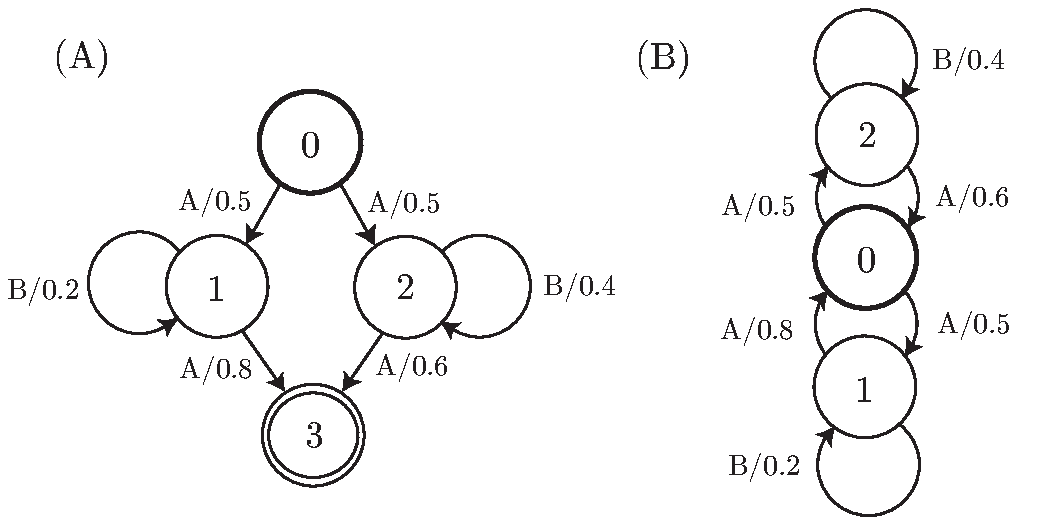
\includegraphics[scale=0.6]{pnfa.pdf}
\caption{Two PNFAs outside the class of PDFAs.  Automaton (A) can be represented by a mixture of two PDFAs, one following the right branch from state 0, the other following the left branch.  Automaton (B), in contrast, cannot be represented by any finite mixture of PDFAs, even though it is nearly the same as (A), but with transition to state 3 replaced by transitions to state 0.}
\label{pnfa}
\end{center}
\end{figure}

% !TEX root = deplump.tex
\section{Previous Work}
\label{section:previous_work}


\subsubsection*{Acknowledgments}

\subsubsection*{References}
\begin{small}
\bibliographystyle{plainnat}
\bibliography{../uber} 
%\input{modrefs}
\end{small}
\end{document}
